

\tikzset{every picture/.style={line width=0.75pt}} %set default line width to 0.75pt        

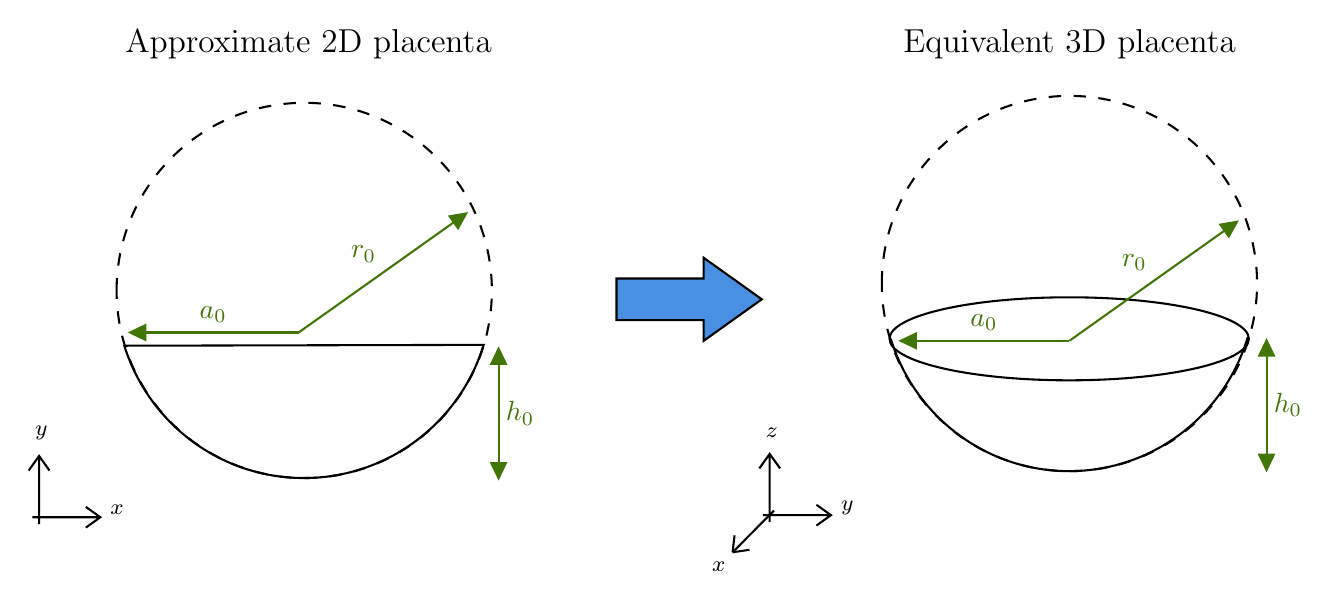
\begin{tikzpicture}[x=0.75pt,y=0.75pt,yscale=-1,xscale=1]
%uncomment if require: \path (0,353); %set diagram left start at 0, and has height of 353

%Shape: Circle [id:dp7318476862281722] 
\draw  [dash pattern={on 4.5pt off 4.5pt}] (67.63,178.06) .. controls (67.63,128.14) and (108.11,87.66) .. (158.03,87.66) .. controls (207.96,87.66) and (248.43,128.14) .. (248.43,178.06) .. controls (248.43,227.99) and (207.96,268.46) .. (158.03,268.46) .. controls (108.11,268.46) and (67.63,227.99) .. (67.63,178.06) -- cycle ;
%Shape: Chord [id:dp48040420887047053] 
\draw   (244.47,204.29) .. controls (232.99,241.87) and (197.88,268.97) .. (156.7,268.44) .. controls (116.48,267.93) and (82.72,241.22) .. (71.36,204.7) -- cycle ;
%Right Arrow [id:dp8732933079811462] 
\draw  [fill={rgb, 255:red, 74; green, 144; blue, 226 }  ,fill opacity=1 ] (308.5,172.33) -- (350.5,172.33) -- (350.5,162.33) -- (378.5,182.33) -- (350.5,202.33) -- (350.5,192.33) -- (308.5,192.33) -- cycle ;
%Shape: Axis 2D [id:dp859721740630015] 
\draw  (27.01,287.34) -- (59.81,287.34)(30.29,257.82) -- (30.29,290.62) (52.81,282.34) -- (59.81,287.34) -- (52.81,292.34) (25.29,264.82) -- (30.29,257.82) -- (35.29,264.82)  ;

%Shape: Axis 2D [id:dp5565758282235733] 
\draw  (379.01,286.34) -- (411.81,286.34)(382.29,256.82) -- (382.29,289.62) (404.81,281.34) -- (411.81,286.34) -- (404.81,291.34) (377.29,263.82) -- (382.29,256.82) -- (387.29,263.82)  ;
%Straight Lines [id:da1846075982859543] 
\draw    (384.33,284.17) -- (364.42,304.21) ;
%Straight Lines [id:da19584630153521942] 
\draw    (372.53,303.03) -- (364.42,304.21) ;
%Straight Lines [id:da589154427729849] 
\draw    (364.42,304.21) -- (365.36,296.07) ;
%Shape: Circle [id:dp8871584214716446] 
\draw  [dash pattern={on 4.5pt off 4.5pt}] (436.3,174.73) .. controls (436.3,124.8) and (476.77,84.33) .. (526.7,84.33) .. controls (576.63,84.33) and (617.1,124.8) .. (617.1,174.73) .. controls (617.1,224.65) and (576.63,265.13) .. (526.7,265.13) .. controls (476.77,265.13) and (436.3,224.65) .. (436.3,174.73) -- cycle ;
%Shape: Ellipse [id:dp5329436538093746] 
\draw   (440.03,201.37) .. controls (440.03,190.32) and (478.78,181.37) .. (526.58,181.37) .. controls (574.39,181.37) and (613.14,190.32) .. (613.14,201.37) .. controls (613.14,212.42) and (574.39,221.37) .. (526.58,221.37) .. controls (478.78,221.37) and (440.03,212.42) .. (440.03,201.37) -- cycle ;
%Shape: Arc [id:dp5756036674906053] 
\draw  [draw opacity=0] (612.58,200.67) .. controls (601.5,237.95) and (567.15,265.13) .. (526.5,265.13) .. controls (486.1,265.13) and (451.93,238.29) .. (440.63,201.37) -- (526.5,174.73) -- cycle ; \draw   (612.58,200.67) .. controls (601.5,237.95) and (567.15,265.13) .. (526.5,265.13) .. controls (486.1,265.13) and (451.93,238.29) .. (440.63,201.37) ;  
%Straight Lines [id:da016157160051171626] 
\draw [color={rgb, 255:red, 65; green, 117; blue, 5 }  ,draw opacity=1 ]   (76,198.33) -- (155.33,198.33) ;
\draw [shift={(73,198.33)}, rotate = 0] [fill={rgb, 255:red, 65; green, 117; blue, 5 }  ,fill opacity=1 ][line width=0.08]  [draw opacity=0] (8.93,-4.29) -- (0,0) -- (8.93,4.29) -- cycle    ;
%Straight Lines [id:da38292659823443675] 
\draw [color={rgb, 255:red, 65; green, 117; blue, 5 }  ,draw opacity=1 ]   (251.67,266.67) -- (251.67,208) ;
\draw [shift={(251.67,205)}, rotate = 90] [fill={rgb, 255:red, 65; green, 117; blue, 5 }  ,fill opacity=1 ][line width=0.08]  [draw opacity=0] (8.93,-4.29) -- (0,0) -- (8.93,4.29) -- cycle    ;
\draw [shift={(251.67,269.67)}, rotate = 270] [fill={rgb, 255:red, 65; green, 117; blue, 5 }  ,fill opacity=1 ][line width=0.08]  [draw opacity=0] (8.93,-4.29) -- (0,0) -- (8.93,4.29) -- cycle    ;
%Straight Lines [id:da046209171807592986] 
\draw [color={rgb, 255:red, 65; green, 117; blue, 5 }  ,draw opacity=1 ]   (234.55,142.07) -- (155.33,198.33) ;
\draw [shift={(237,140.33)}, rotate = 144.62] [fill={rgb, 255:red, 65; green, 117; blue, 5 }  ,fill opacity=1 ][line width=0.08]  [draw opacity=0] (8.93,-4.29) -- (0,0) -- (8.93,4.29) -- cycle    ;
%Straight Lines [id:da11320604093348186] 
\draw [color={rgb, 255:red, 65; green, 117; blue, 5 }  ,draw opacity=1 ]   (447.33,202.33) -- (526.67,202.33) ;
\draw [shift={(444.33,202.33)}, rotate = 0] [fill={rgb, 255:red, 65; green, 117; blue, 5 }  ,fill opacity=1 ][line width=0.08]  [draw opacity=0] (8.93,-4.29) -- (0,0) -- (8.93,4.29) -- cycle    ;
%Straight Lines [id:da4015288476308778] 
\draw [color={rgb, 255:red, 65; green, 117; blue, 5 }  ,draw opacity=1 ]   (605.89,146.07) -- (526.67,202.33) ;
\draw [shift={(608.33,144.33)}, rotate = 144.62] [fill={rgb, 255:red, 65; green, 117; blue, 5 }  ,fill opacity=1 ][line width=0.08]  [draw opacity=0] (8.93,-4.29) -- (0,0) -- (8.93,4.29) -- cycle    ;
%Straight Lines [id:da4715079348134419] 
\draw [color={rgb, 255:red, 65; green, 117; blue, 5 }  ,draw opacity=1 ]   (621.67,262.67) -- (621.67,204) ;
\draw [shift={(621.67,201)}, rotate = 90] [fill={rgb, 255:red, 65; green, 117; blue, 5 }  ,fill opacity=1 ][line width=0.08]  [draw opacity=0] (8.93,-4.29) -- (0,0) -- (8.93,4.29) -- cycle    ;
\draw [shift={(621.67,265.67)}, rotate = 270] [fill={rgb, 255:red, 65; green, 117; blue, 5 }  ,fill opacity=1 ][line width=0.08]  [draw opacity=0] (8.93,-4.29) -- (0,0) -- (8.93,4.29) -- cycle    ;

% Text Node
\draw (63.19,283.86) node [anchor=west] [inner sep=0.75pt]  [font=\footnotesize]  {$x$};
% Text Node
\draw (31.33,251.41) node [anchor=south] [inner sep=0.75pt]  [font=\footnotesize]  {$y$};
% Text Node
\draw (383.33,250.41) node [anchor=south] [inner sep=0.75pt]  [font=\footnotesize]  {$z$};
% Text Node
\draw (415.19,282.86) node [anchor=west] [inner sep=0.75pt]  [font=\footnotesize]  {$y$};
% Text Node
\draw (362.42,307.61) node [anchor=north east] [inner sep=0.75pt]  [font=\footnotesize]  {$x$};
% Text Node
\draw (160.06,68.19) node [anchor=south] [inner sep=0.75pt]  [font=\large] [align=left] {\begin{minipage}[lt]{140.17pt}\setlength\topsep{0pt}
\begin{center}
Approximate 2D placenta
\end{center}

\end{minipage}};
% Text Node
\draw (526.73,68.19) node [anchor=south] [inner sep=0.75pt]  [font=\large] [align=left] {\begin{minipage}[lt]{128.61pt}\setlength\topsep{0pt}
\begin{center}
Equivalent 3D placenta
\end{center}

\end{minipage}};
% Text Node
\draw (114.17,194.93) node [anchor=south] [inner sep=0.75pt]  [color={rgb, 255:red, 65; green, 117; blue, 5 }  ,opacity=1 ]  {$a_{0}$};
% Text Node
\draw (253.67,237.33) node [anchor=west] [inner sep=0.75pt]  [color={rgb, 255:red, 65; green, 117; blue, 5 }  ,opacity=1 ]  {$h_{0}$};
% Text Node
\draw (194.17,165.93) node [anchor=south east] [inner sep=0.75pt]  [color={rgb, 255:red, 65; green, 117; blue, 5 }  ,opacity=1 ]  {$r_{0}$};
% Text Node
\draw (485.5,198.93) node [anchor=south] [inner sep=0.75pt]  [color={rgb, 255:red, 65; green, 117; blue, 5 }  ,opacity=1 ]  {$a_{0}$};
% Text Node
\draw (565.5,169.93) node [anchor=south east] [inner sep=0.75pt]  [color={rgb, 255:red, 65; green, 117; blue, 5 }  ,opacity=1 ]  {$r_{0}$};
% Text Node
\draw (623.67,233.33) node [anchor=west] [inner sep=0.75pt]  [color={rgb, 255:red, 65; green, 117; blue, 5 }  ,opacity=1 ]  {$h_{0}$};


\end{tikzpicture}
